\documentclass[a4paper,12pt,obeyspaces,spaces,hyphens]{article}

\def \trainingtype{onsite}
\def \agendalanguage{french}

\input{agenda/preempt-rt.inc}

\usepackage{agenda}

\begin{document}

\feshowtitle

\feagendasummaryitem{Title}{
  {\bf \trainingtitle{}}
}
\feagendasummaryitem{Objectifs\newline opérationnels}{
  \traininggoals{}
}
\feagendasummaryitem{Duration}{
  \feshowduration{}
}
\onsitepedagogics{50}{50}
\feagendasummaryitem{Formateur}{
  \trainers{}
}
\feagendasummaryitem{Langue}{
  \traininglanguages{}
}
\feagendasummaryitem{Audience}{
  \trainingaudience{}
}
\feagendasummaryitem{Pré-requis}{
  \trainingprerequisites{}
}
\feagendasummaryitem{Équipement nécessaire}{
  \requiredequipment{}
}
\certificate{}
\disabilities{}

\feagendatwocolumn
{Plateforme matérielle pour les travaux pratiques}
{
  Carte {\bf STMicroelectronics STM32MP157D Discovery Kit~1}
  \begin{itemize}
  \item Processeur STM32MP157D (dual Cortex-A7) de STMicroelectronics
  \item Alimentation par USB
  \item 512 MB DDR3L RAM
  \item Ethernet Gigabit
  \item 4 ports USB 2.0 hôte
  \item 1 port USB-C OTG
  \item 1 slot Micro SD
  \item Debugger ST-LINK/V2-1
  \item Connecteurs compatibles Arduino
  \item Codec audio, boutons, LEDs
  \end{itemize}
}
{}
{
  \begin{center}
    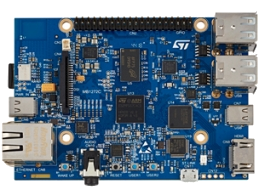
\includegraphics[width=5cm]{../slides/discovery-board-dk1/discovery-board-dk1.png}
  \end{center}
}

\section{1\textsuperscript{ère} journée - Matin}

\feagendaonecolumn
{Cours - Introduction au comportement temps-réel et au déterminisme}
{
  \begin{itemize}
  \item Définition d'un système d'exploitation temps-réel
  \item Spécificigés des systèmes multi-tâches
  \item Principaux patterns de verrouillage et de gestion des priorités
  \item Aperçu des systèmes temps-réel existants
  \item Approches pour apporter un comportement temps-réel à Linux
  \end{itemize}
}

\feagendatwocolumn
{Cours - Le patch {\em PREEMPT\_RT}}
{
  \begin{itemize}
  \item Histoire et avenir du patch {\em PREEMPT\_RT}
  \item Améliorations temps-réel provenant de {\em PREEMPT\_RT} dans le noyau Linux officiel
  \item Fonctionnement interne de {\em PREEMPT\_RT}
  \item Gestion des interruptions: interruptions threadées, softirqs
  \item Primitives de verouillage: mutexes et spinlocks, spinlocks avec sommeil
  \item Modèles de préemption
  \end{itemize}
}
{TP - Compiler un noyau Linux avec {\em PREEMPT\_RT}}
{
  \begin{itemize}
  \item Télécharger le noyau Linux et appliquer le patch {\em PREEMPT\_RT}
  \item Configurer le noyau Linux
  \item Démarrer le kernel sur une plateforme matérielle
 \end{itemize}
}

\section{1\textsuperscript{ère} journée - Après-midi}

\feagendaonecolumn
{Cours - Configuration et limites du matériel pour le temps-réel}
{
  \begin{itemize}
  \item Interruptions et firmware
  \item Interaction avec les fonctionnalités de gestion d'énergie:
    gestion dynamique de la fréquence du CPU et états de sommeil
  \item DMA
  \end{itemize}
}

\feagendatwocolumn
{Cours - Outils: Benchmarking, Stress et Analyse}
{
  \begin{itemize}
  \item Benchmarking avec {\em cyclictest}
  \item Stress du système avec {\em stress-ng} et {\em hackbench}
  \item L'infrastructure de {\em tracing} du noyau Linux
  \item Analyse de la latence et de l'ordonnancement avec {\em
      ftrace}, {\em kernelshark} ou {\em LTTng}
  \end{itemize}
}
{TP - Outils: Benchmarking, Stress et Analyse}
{
  \begin{itemize}
  \item Utilisation des outils de benchmark et de stress
  \item Techniques classiques de benchmarking
  \item Benchmarking et configuration de la plateforme matérielle
  \end{itemize}
}

\section{2\textsuperscript{ème} journée - Matin}

\feagendaonecolumn
{Cours - Infrastructures du noyau Linux et configuration}
{
  \begin{itemize}
  \item Bonnes pratiques pour le développement de drivers noyau Linux
    pour des systèmes temps-réel
  \item Politiques d'ordonnancement et priorités: {\em SCHED\_FIFO},
    {\em SCHED\_RR}, {\em SCHED\_DEADLINE}
  \item Affinité CPU et IRQ
  \item Gestion mémoire
  \item Isolution des CPUs avec {\em isolcpus}
  \end{itemize}
}

\feagendaonecolumn
{Cours - Patterns de développement d'applications temps-réel}
{
  \begin{itemize}
  \item API POSIX pour les applications temps-réel
  \item Gestion et configuration des threads
  \item Gestion mémoire: allocation mémoire et verouillage mémoire, gestion de la pile
  \item Patterns de verrouillage: mutexes, héritage de priorité
  \item Communication inter-processus (IPC)
  \item Signalisation
  \end{itemize}
}

\section{2\textsuperscript{ème} journée - Après-midi}

\feagendaonecolumn
{TP - Débugger une application de démonstration}
{
  \begin{itemize}
  \item Créer une application de démonstration déterministe
  \item Utiliser l'infrastructure de {\em tracing} pour identifier la source de latence
  \item Apprendre à utiliser l'API POSIX pour gérer les threads, le verouillage, la mémoire
  \item Apprendre à utiliser l'affinité CPU et configurer la politique d'ordonnancement
  \end{itemize}
}

\feagendaonecolumn
{Questions / réponses}
{
  \begin{itemize}
  \item Questions / réponses avec les participants autour du noyau Linux
  \item Des présentations supplémentaires s'il reste du temps, selon les sujets
	qui intéressent le plus les participants.
  \end{itemize}
}

\end{document}
